\section{Queen}

Our front-end component, also built on the NodeJS framework pulls all of the
components of Hive together to provide a real-time, visually rich experience.

We used the Express\cite{express} library in NodeJS to build an MVC framework for the UI
to
keep in line with our design style throughout the rest of the project. This has
lead to a clean, modular codebase that has very little duplication of code.
The most important decision designing Queen was to ensure that all data
transferred to the front-end would happen in real-time. In order to enable this
we took advantage of the socket.io\cite{socket} library to have web-sockets that allow
client(front-end) to server(Queen back end server) communication.

Like the rest of our components Queen uses RabbitMQ to provide inter-component
communication. The flow for communication with other components is described
here
using a user performing a search as an example:

\begin{enumerate}
  \item The search terms are passed from the UI as a JSON object back to
  Queens
  server via a web-socket.
  \item Queen server then passes this data onto the appropriate Hive
  component
  via RabbitMQ, using either a remote procedure call or
  publish/subscribe model
  as appropriate.
  \item The Hive component (in this case Honeycomb) will then
  return the data to
  Queen server.
  \item The exact data that is required for the
  front-end is extracted and
  passed back up to the UI via a web-socket.
\end{enumerate}

If we request data using a publish/subscribe model, then
every time the Queen
server receives data on the subscribe queue it can push
that data back up to the
front-end using a web-socket. This means that the UI
always has all of the
information available to it and the browser will not
freeze as it would if we
were using a RESTful/polling approach to getting new
data to the UI.

Queen enables multiple users to all be using the service
at once. The principle
for multiple users is to store queries/alerts that the
user wants to access next
time they use the system, also to store a list of
Devices associated to the user
to be used by our iOS application. To store this data
persistently Queen also uses
MongoDB.

\vspace{10 mm}
\graphicspath{{./pics/}}
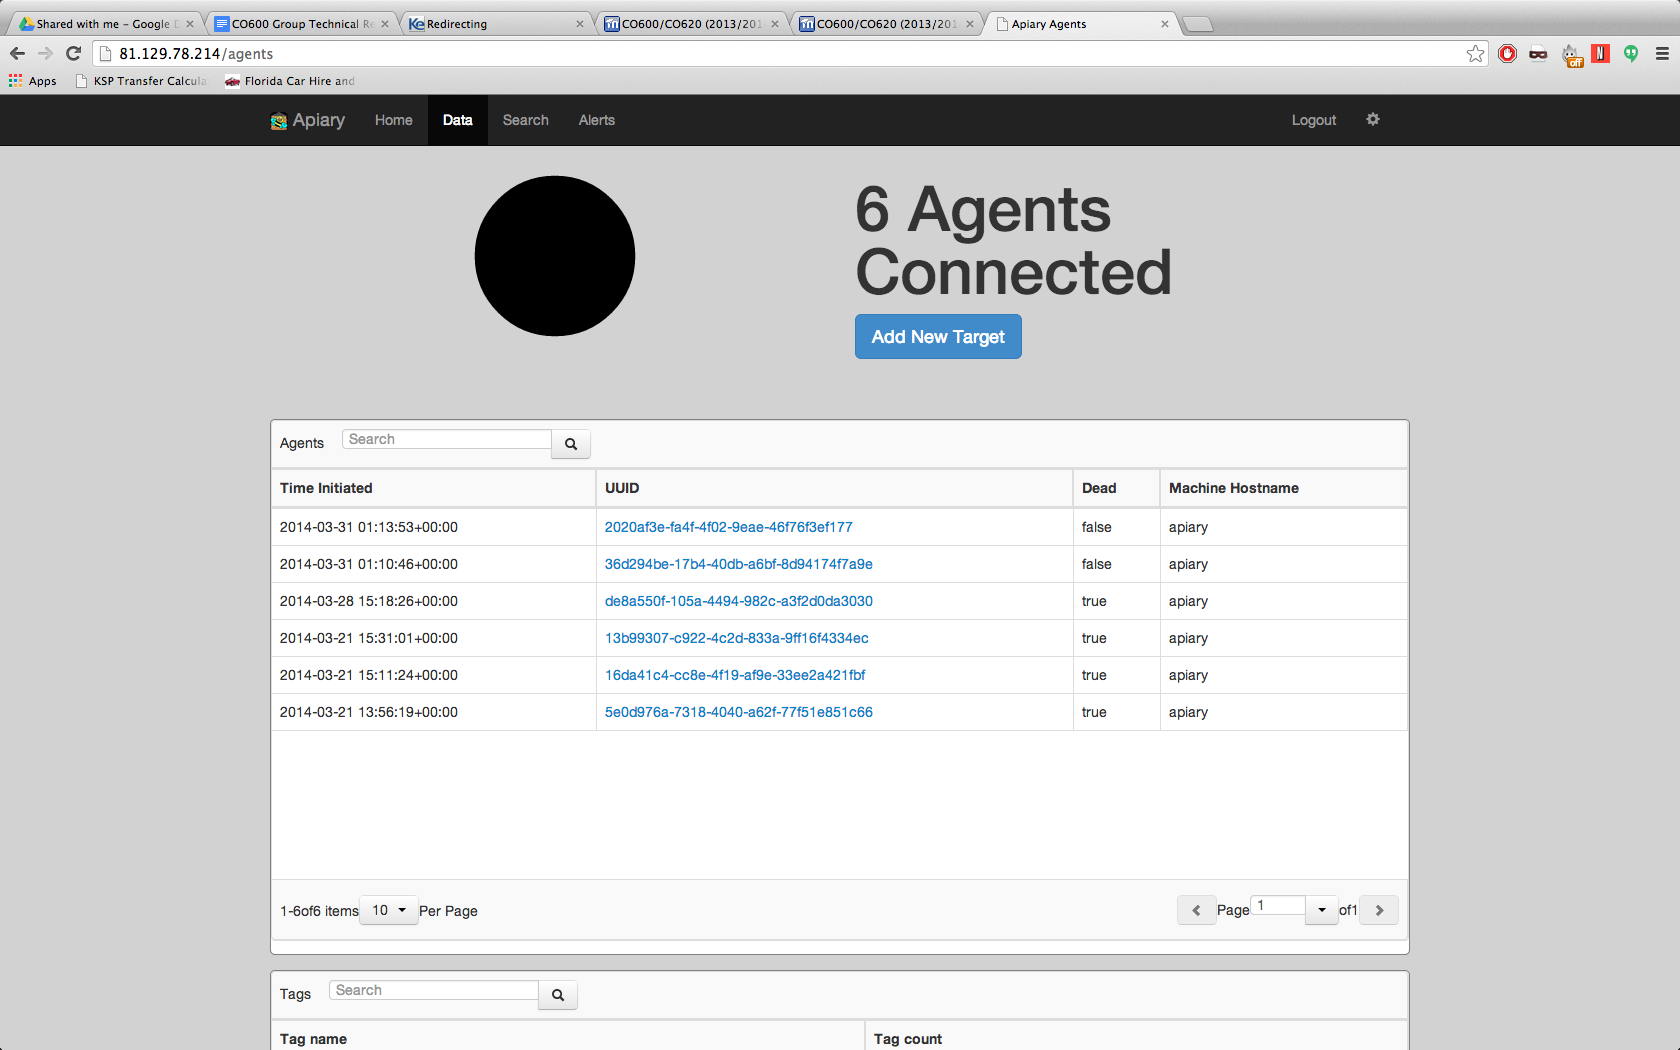
\includegraphics[width=8cm, keepaspectratio]{data.png}
\vspace{10 mm}

Just as we did with the Bee agents we wanted to keep
Queen configuration as
simple as we could. The configuration options as such
are kept to just the IP
address of the RabbitMQ server that all of the other
components are talking on and
the IP address of the mongo server. By having the IP
address of the mongo server
as a configuration option Queen can either be running
its own mongo server or
use the existing one setup for Hive.

Rich visualisations were another main goal in designing
Queen, due to our
experience using the d3js\cite{d3} visualisation library we
naturally decided to use
this. It has enabled us to use visualisations such as
sparkline graphs to map
event rates in the system and pie charts to compare search
results. From a
human computer interaction (HCI) point of view this gives
the user access to the
same data in a more meaningful form, and that data can be
accessed at a glance
rather than reading copious amounts of text to come to the
same conclusion.

\vspace{10 mm}
\graphicspath{{./pics/}}
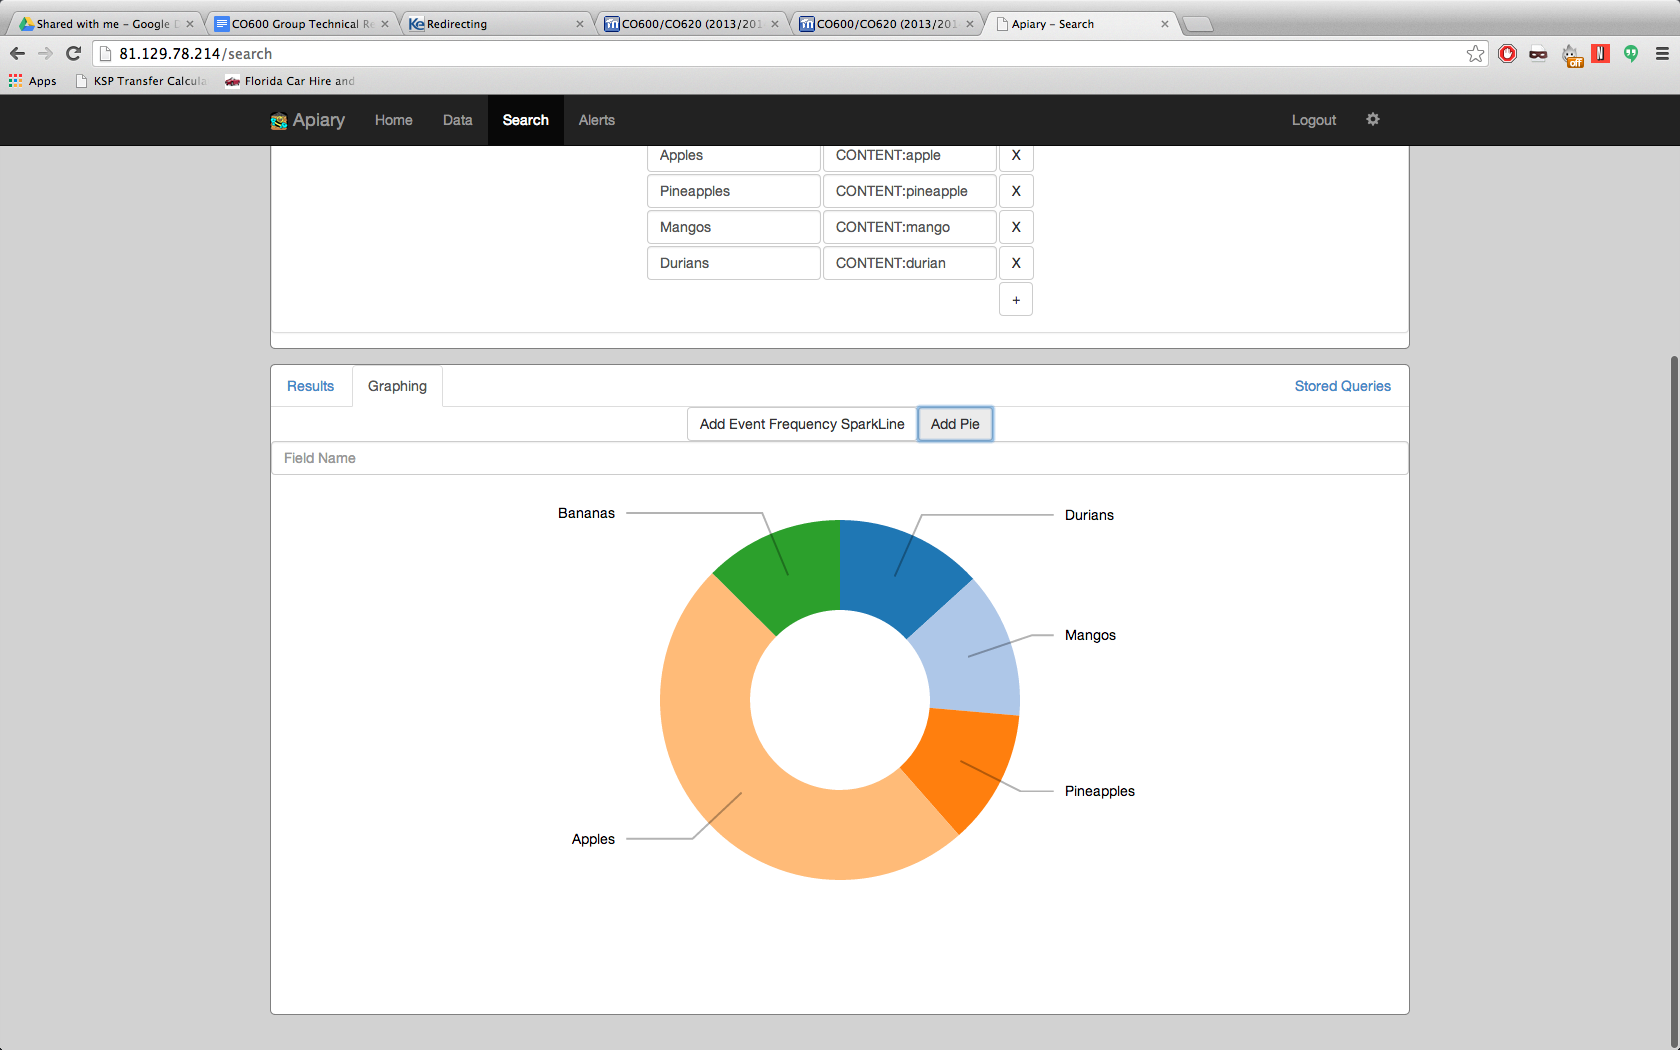
\includegraphics[width=8cm, keepaspectratio]{search.png}
\vspace{10 mm}

Due to the quantity of data that can come back from search
results it was
important not only to visualise this in graph form but
also allow users to
filter the actual log entries live in the browser opposed
to sending of another
more refined query to Hive. In order to do this we put all
data that we desire
to be searchable in a datagrid from the FuelUX\cite{fuelux} library
which provides instant
searching for all data in the datagrid.

Key to being able to graph data, was being able to infer
schema onto our logs and break queries down into fields. For
this we came up with a system whereby a query could be
broken into subqueries, and each of these subqueries could
represent a member of a field. This allowed us to then take
the results, partition them, and graph the various members
against one another. The subqueries are made independently,
and the results collated and returned to the browser. This
is what allows us to really gain value from otherwise
unorganised log data, as you can now start to make
meaningful analysis.

